\chapter{Classification methods }
In previous chapter, we introduce a method to remove the unexpected object. In this chapter, we will propose a method to obtain the features what we are interested in and the method to detect the landmarks on the insect. This method was proposed by Palaniswamy$^{\cite{palaniswamy2010automatic}}$. The processes can be discuss in follow steps:
\begin{enumerate}
\item Extracting the features:
\item Constructing and comparing the pairwise geometric histogram
\item Estimating the pose by the probabilistic Hough transform
\item Detecting the landmarks by template matching
\end{enumerate}
\section{Preprocessing image and feature extraction}
To obtain the good result, before extracting the features in the image, we need to pre-process the image with a appropriate technique to reduce the noise as well as enhance the features that we care. 
Feature extraction is a process extracting interested features from digital image. The expect result in this result is list of approximate lines which use to construct the pairwise geometric histogram. \\[0.2cm]
The process mainly separate into two stages: Firstly, we pre-process image. In this stage, we reduce the noise in image by finding a threshold value and apply the thresholding technique to obtain the interested features. Secondly, we extract the features based on the edge segmentation. By applying the appropriate technique to obtain the step edges and broken the edges into approximate lines.
\subsection{Preprocess image}
In this application, we use the thresholding technique to pre-process the image. In thresholding technique, with a threshold value ``t", we can decrease the noise and obtain the interested features. The threshold value can be defined by the histogram analysis.\\[0.2cm]
Based on the histogram of the original image, we compute the mean and median of this histogram. With the histogram obtained, we split it into two parts: the first part begin from the bin 0 to the limit value (the limit value is smallest value between mean and median); the second part, starting from the limit value to the end of histogram. For each part, we find the maximum, minimum value and calculating the mean of it. The value ``t" obtained by the mean of two mean values in two parts of histogram.\\
With the threshold value ``t", we apply the threshold technique to pre-process image in the CV\_THRESH\_BINARY mode (keep the pixel has value greater than threshold value).\\
\IncMargin{1em}
\begin{algorithm}[H]
\Indm 
\KwData{inputImage: the input image}
\KwResult{outputImage: the image after processing}
\Indp
Convert the input image into gray scale image\;
Calculate the histogram on gray scale image and store the result in $histogram$ variable \;
Compute the $mean$ value and $median$ value of histogram\;
$limit \leftarrow (mean > median$ ? $median : mean)$\;
$limitSub \leftarrow ((limit >= 120)$ ? $(limit - 25) : (limit - 5))$\;
Declare some variables: $int$ $imax \leftarrow -1, max \leftarrow -1$\;
\For{$i \leftarrow$ 0 to $limitSub$}{
	\If{$histogram[i]$ $>$ $max$}{
		$max$ = $histogram[i]$\;
		$imax$ = $i$\;
	}
}
Declare some variables: $int$ $imin \leftarrow -1, min \leftarrow max$\;
\For{$k \leftarrow$ imax to $limit$}{
	\If{$histogram[k]$ $<$ $min$}{
		$min$ = $histogram[k]$\;
		$imin$ = $k$\;
	}
}
Declare some variables: $int$ $max2 \leftarrow -1, imax2 \leftarrow -1$\;
\For{$j \leftarrow limit $ to $end\_of\_histogram$}{
	\If{$histogram[j]$ $>$ $max2$}{
		$max2$ = $histogram[j]$\;
		$imax2$ = $j$\;
	} 
}
$middle1 \leftarrow (imax1 + imin)/2$ \;
$middle2 \leftarrow (imax2 + imin)/2$ \;
$middle \leftarrow (middle1 + middle2)/2$ \;
Apply the threshold with threshold value is $middle$\;
\caption{Algorithm to preprocess image}
\end{algorithm}\DecMargin{1em}
\subsection{Feature extraction}
After apply the threshold to pre-process image, we apply the Canny algorithm to detect the step edges, which incorporates non-maximal suppression and hysteresis thresholding. In Canny, the importance parameters are two threshold values and aperture size for the Sobel operator, it decides the pixels kept. The threshold value used in Canny algorithm also the value used in the previous step, and the ratio between lower threshold and upper threshold is 1.5 : 3 (follows the article \cite{palaniswamy2010automatic}). In implementation, the Canny operation used from OpenCV library\footnote{http://docs.opencv.org/modules/imgproc/doc/feature\_detection.html\#canny}, and the parameters need to put into Canny are:
\begin{itemize}
\item source: the input image (in grayscale mode)
\item destination: the output image
\item low\_thresh: the first (lower) threshold value
\item hight\_thresh: the second (upper) threshold value
\item kernel\_size: size of kernel, aperture for the Sobel operator
\end{itemize}
The Canny algorithm is not aware of actual edges, the edge detecting was based on the Sobel operator, extracted with non-maximal suppression. So, to obtain the expect result, we  need to apply another technique to obtain the step edges. The \textbf{findContours} was chosen for this aim, the result is a vector of the edges, and each edge was presented by a vector of the points. Like the Canny, the \textbf{findContours} also used from OpenCV library \footnote{http://docs.opencv.org/modules/imgproc/doc/structural\_analysis\_and\_shape\_descriptors.html\#findcontours} and the parameters used in this operation as follows:
\begin{itemize}
\item source: the binary input image
\item contours: the output. Each contours is stored in a vector of points.
\item hierarchy: optional output vector, containing information about the image topology.
\item mode: contours retrieve mode
\item method: contours approximation method
\item offset: optional offset by which every contour point is shifted.
\end{itemize}
\subsection{Edge segmentation}
The geometric relation can not constructed from the edges, it always construct from the relation of basic geometric objects, such as the lines.  In fact, any arbitrary edge can be represented by a set approximate lines. Instead of representing an edge, we can represent a set of approximate lines of it. This way also useful when we want presentation the edges or describe the relation between it. With the set of step edges was obtained from find contours (the image structure). In this step, we will segment it to approximated lines. The method to segment the edges is a recursive algorithm$^{\cite{riocreux1994analysis}}$ but it have some change in the ``stop condition" of algorithm to easy process, as follows:
\begin{itemize}
\item Establish a line \textit{``l"} between two endpoints of edge.
\item For each point on edge, we compute the perpendicular distance from it to the line l and keep the point which has the maximum perpendicular distance.
\item If the maximum perpendicular distance from a point on edge to the line \textit{l} is greater than $\alpha$, then the edge is split at this point. The value chosen for $\alpha$ in the program is 3 ($\alpha = 3$).
\item Reprocess both parts which was obtained from step 3.
\item The algorithm continues until all edges fragments are represented.
\end{itemize}
The algorithm is presented as follows:\\
\IncMargin{1em}
\begin{algorithm}[H]
\Indm 
\KwData{listPoints: list of points which presented the edge}
\KwResult{Queue of ``step" points on the edge}
\Indp
Declare the first endpoint: $p0 \leftarrow listPoints[0]$\;
Declare the second endpoint: $pend \leftarrow listPoints[size - 1]$, \textit{size} is the size of \textit{listPoints}\;
Set up a straight line between the two endpoints $p0, pend$ (line $d$)\;
Initialization the max value: $maxDistance  \leftarrow 0 $\;
Declare a ``split point": $imax \leftarrow 0$ \; 
Declare a variable: $distance \leftarrow 0$\;

\For{ point $p$ in $listPoints$}{
	$distance \leftarrow$ from $p$ to line $d$\;
	\If{distance $>$ max\_distance}{
		$maxDistance$ $\leftarrow$ $distance$\;
		$imax$ $\leftarrow$ position of $p$\;
	}
}
\If{$maxDistance$ $>$ 3 }{
	split the list of points at $imax$ and put into 2 parts $(part1, part2)$\;
	Pre-process on $part1$\;	
	Pre-process on $part2$\;
}
\If {$p0$ does not exist in result queue}{
	push $p0$ into queue\;\tcp{queue is a variable of class}
}
\If {$pend$ does not exist in result queue}{
	push $pend$ into queue\;\tcp{queue is a variable of class}
}
\caption{Algorithm to segment an edge}
\end{algorithm}\DecMargin{1em}
\section{Pairwise geometric histogram}
Pairwise geometric histogram(PGH) is used to encode the relative information between a line and a set of lines in an object. Therefore, an object can represented by a set of PGH. From the set of PGH, we can reconstructed the object or compare with another object. In this section, we will mention the constructing a PGH for an object based on the geometrical relationship and compute the similar distance between two objects.

\subsection{Pairwise geometric histogram}
The PGH is constructed on the geometric features between lines relative. The geometric features are characteristic which can describe the geometric shape such as angle, the length of line, perpendicular between two lines,.... For the shape representation, the relative angle and perpendicular distance is geometrical features useful. \\
The proceed to construct the PGH was described in below:
\begin{itemize}
\item Choose the reference line (called reference line, another called object line)
\item Compute the angle between two lines
\item Calculate the perpendicular distance from two endpoints of object line to the reference line (assigned dmin and dmax).
\item Recording the perpendicular distance and angle relative between two lines.
\end{itemize}
Example \footnote{Images extract from the article \cite{palaniswamy2010automatic}}:\\
\begin{figure}[h!]
\centering
\subfloat[The geometric relationship between two lines]{\label{fig:example_1}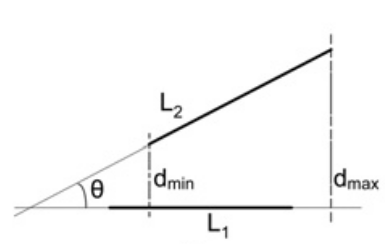
\includegraphics[width=0.4\textwidth]{./images/PGH_geo}}~~
\subfloat[The pairwise geometric histogram ]{\label{fig:example_2}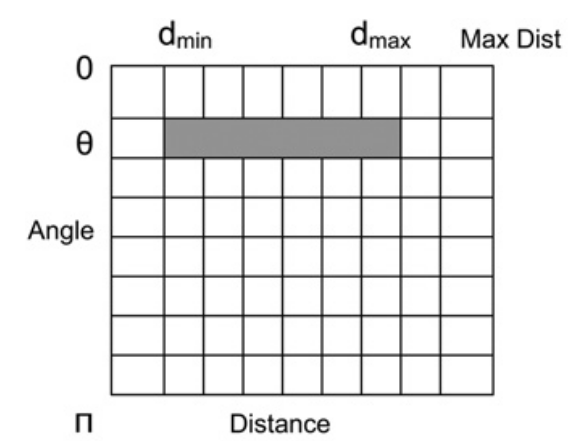
\includegraphics[width=0.4\textwidth]{./images/PGH}}
\caption{The geometric features and the PGH}
\label{fig:figure_31}
\end{figure}
\\[0.3cm]The frequency of the geometric features is recorded as a two dimensional histogram with an angle axis (0 - $\pi$) and distance axis (range of perpendicular distance, $d_{max}$ is the maximum distance on all distance of two arbitrary lines). The entries on PGH describe the geometric relationship between the reference line and the object lines. The blurring of entry along the axis regarding the true position and orientation of each object lines for reference line.
\\The full object representation is constructed by recording the PGH for each line within object. If the object is defined by n lines, the full shape representation will composed of n pairwise geometric histograms.\\
This method still good when we apply some variants on the image, such as translate or rotate the image because the angle and perpendicular distance between a pair of lines is invariant.
\subsection{Histogram matching}
``The histogram matching enables robust classification of shape features by finding similarity between the scene and reference model"$^{\cite{palaniswamy2010automatic}}$. The similar between two models can obtain via the similar distance, which was computed by comparing their probability distribution on geometric histogram. In program, each image was represented by a comprises of many geometric histograms and using the Bhattacharyya metric to determine the similar distance between two models $^{\cite{palaniswamy2010automatic}}$. In general, we have normalize the histograms before comparing. The form of Bhattacharryya metric used to compute the degree of 2 model:
\begin{center}
\begin{equation} \label{eq:1}
d_{Bhattacharyya} (H_{i}H_{j}) = \sum\limits_{\theta}^{\pi}\sum\limits_{d}^{d_{max}}\sqrt{H_{i}(\theta,d)H_{j}(\theta,d)}
\end{equation}
\end{center}
The significance of parameters in the formula \ref{eq:1}, as follows:
\begin{itemize}
\item $\theta$: angle value, range of $\theta$ in angle axis from 0 to $\pi$.
\item $d$: the perpendicular distance, range of d in perpendicular distance from 0 to the maximum distance of arbitrary lines of shape.
\item $H_{i}(\theta,d)$ is an entry at row $\theta$ and column d in histogram of image \textit{i}
\item $H_{j}(\theta,d)$ is an entry at row $\theta$ and column d in histogram of image \textit{j}
\end{itemize}
By the default, the range of angle axis from 0 to 180 degree (correspondence with 180 degree). Based on the accuracy of program, we can increase the range of angle axis. This design allow increase the range of angle axis to several time with default value. Example, the table below show the result when calculating Bhattacharyya distance between image \textit{Md 028.JPG} and some images with difference accuracy:
\begin{center}
\begin{tabular}{|l|l|c|c|c|c|c|c|}
\hline
Reference image & Scene image & 180 & 2 * 180 & 4 * 180 & 6 * 180 \\ \hline
Md 028.JPG & Md 001.JPG & 0.977953 & 0.964167 & 0.93861 & 0.91471 \\ \hline
Md 028.JPG & Md 005.JPG & 0.96479 & 0.943657 & 0.906444 & 0.871756  \\ \hline
Md 028.JPG & Md 010.JPG & 0.976241 & 0.958061 & 0.925943 & 0.896445 \\ \hline
Md 028.JPG & Md 027.JPG & 0.980728 & 0.968233 & 0.945442 & 0.92485 \\ \hline
\end{tabular}
\end{center}
Besides the Bhattacharyya metric, we can also choose another metric to matching the histograms, such as: \textbf{Chi-squared} metric and \textbf{Intersection} metric. The forms was presented as below:\\
\textbf{Chi-squared metric:}
\begin{center}
\begin{equation}\label{eq:2}
d_{Chi-squared} (H_{i}H_{j}) = \frac{\sum\limits_{\theta}^{\pi}\sum\limits_{d}^{d_{max}}(\frac{(H_{i}(\theta,d) - H_{j}(\theta,d))^{2}}{(H_{i}(\theta,d) + H_{j}(\theta,d))})}{2}
\end{equation}
\end{center}
\textbf{Intersection metric}
\begin{center}
\begin{equation}\label{eq:3}
d_{Intersection} (H_{i}H_{j}) = \sum\limits_{\theta}^{\pi}\sum\limits_{d}^{d_{max}}min(H_{i}(\theta,d), H_{j}(\theta,d))
\end{equation}
\end{center}
The significance of parameters in equation (\ref{eq:2}) and (\ref{eq:3}) is similar with (\ref{eq:1}). For the Bhattacharyya and Intersection metric, the perfect match is 1 and the total mismatch is 0. The result is opposite to Chi-squared metric (0 for perfect match and 1 for total mismatch).\\[0.2cm]
Hence, depend on the purpose of comparison will choose a suitable comparing method. In this program, we want to try on three method to have a general view result when matching the histograms.
\subsection{Statistical the matching result}
Based on the result of matching histogram. In this step, we will do a statistical to classify the result into other groups.
































